\newpage
\section{Multi-Party Computation (MPC)}

The first approach to ensuring trust in the Sphinx header is to prevent user manipulation by decentralizing the header construction to Trusted Third Parties (TTP) through the use of Multi-Party Computaftion (MPC).

We consider TTPs as \textit{honest-but-curious}.\tothink{What if malicous TTP...}
This means that they follow the protocol correctly but may attempt to infer additional information from the data they process.
Our design aims to ensure that TTPs must not be able to infer any information about the shared secrets $s_i$ nor the mixnodes involved in the path, even when TTP are colliding (assuming that at least one TTP remains honest).
\newline


% Overall path selection:
% 1) Users choose the path
% 2) TTP randomly choose the path (without knowing it)

% Overall schema 
% 1̶)̶ ̶O̶n̶e̶ ̶T̶T̶P̶ ̶p̶e̶r̶ ̶l̶a̶y̶e̶r̶
% 2) TTP do a layer, then aggregate, then next layer  => What if user send h(s_i) ?! (TODO)
% 3) TTP do the whole computation then aggregate
To decentralize the construction of the Sphinx header, we first examined how to partition and distribute the computation. 
Three approaches were considered.

The first and most naive approach involves that each TTP computes a different layer of the header. 
This approach reveals two consecutive nodes in the path and one of the corresponding shared secrets ($s_i$) at each TTP, leading to serious security concerns in the case of collusion.

In a second approach, the user sends to each TTP a piece of the destination address.
Each TTP computes the same layer on its partial destination.
The resulting partial headers of this layer are aggregated to compute the integrity tag. 
This process is repeated layer by layer. 
However, computing the integrity tag at the end of each layer requires knowledge of the shared secret $s_i$. 
\tothink{User could send $h(s_i)$ to TPP such that it could computes the integrity check without getting useful information...}
If a TTP does it, it reintroduces the same problem as the first approach.
If the user does it, he could potentially cheat.

The third and retained approach is similar to the second one.
Instead of partial computations at each layer, each TTP computes a full Sphinx header using only its assigned partial destination. 
These partial headers are then returned to the user, who aggregates them to produce the final Sphinx header.
Although this approach requires less interaction with the TTPs, it introduces additional constraints as discussed in section \toref{ref section}.

The overall decentralized scheme is illustrated in Figure \ref{fig:overall_schema}. 
The user begins by splitting the destination into several parts, such that their combination (e.g., via XOR) reconstructs the original address. 
Each part is sent to a different TTP, along with the required cryptographic material. 
The TTPs independently generate Sphinx headers using a modified version of the protocol. \toref{(see section ...)} 
These partial headers are then returned to the user, who aggregates them to form the final Sphinx header, ready for transmission through the mixnet.

\begin{figure}[H]
    \centering
    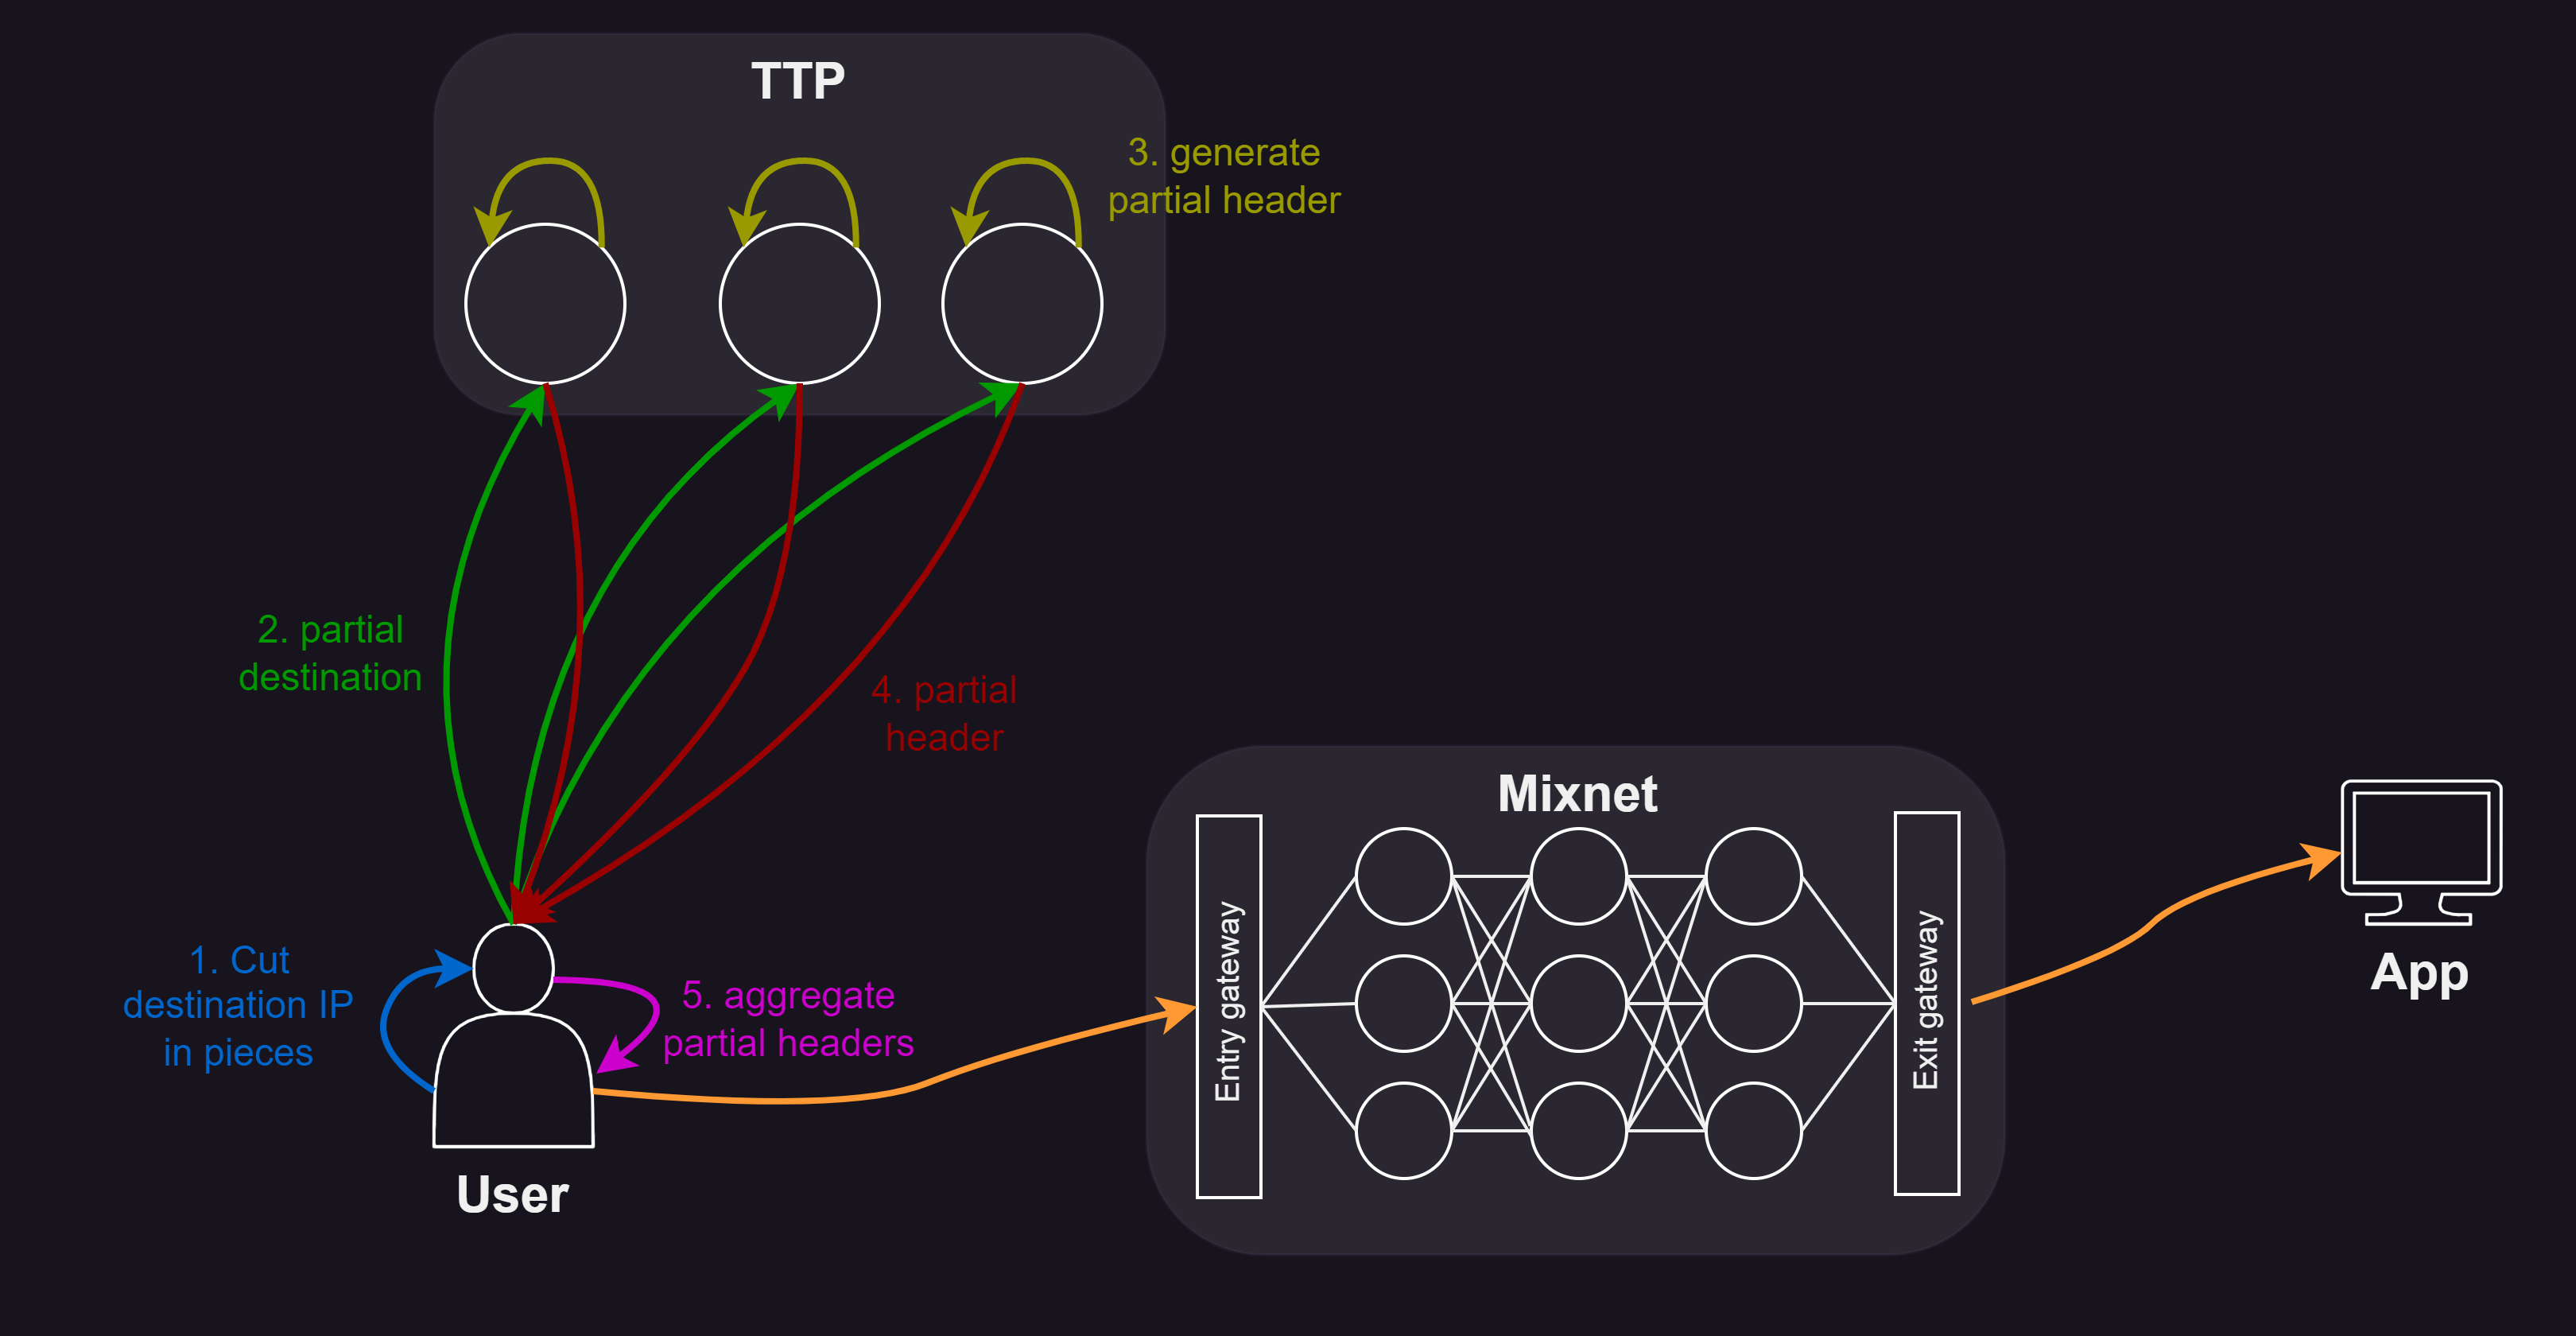
\includegraphics[width=1\linewidth]{Images/sphinx_ttp.png}
    \caption{Overview of the decentralized scheme}
    \label{fig:overall_schema}
\end{figure}

%%%%%%%%%%%%%%%
%One major challenge in decentralizing the original sphinx schema (Figure \ref{fig:header_cipher}) lies in the integrity tag, which is computed as the HMAC of the header $\beta_i$ using shared secret $s_i$. 
%To ensure security, no third party should have access to $s_i$, as collusion among third parties could lead to the recovery of all $s_i$, enabling them to decrypt the header and payload.
%To address this, third parties could compute a portion of the HMAC using a fragment of the shared secret $s_i$, and then combine these partial HMACs to produce the final HMAC. 
%This approach would require a hash function with homomorphic properties, which inherently weakens the collusion resistance and potentially compromises the second pre-image resistance of a secure hash.
%%%%%%%%%%%%%%%

The main issue with the choosen approach is that we have to compute integrity tag on partial header such 
that combining those partial integrity tag gives the integrity tag of the final header.
However, even if breaking this homomorphic hash is feasible, if it remains computationally hard enough (e.g., requiring several hours), it could still be considered sufficiently secure for our purposes.
% TODO: VERIFY WHY NEED TO BE PER CHUNK
% What append if size secret bigger than chunk size (more random ?)


% ALPHA - 3 possibilities
% 1) Sending 1 alpha that is derived at each mixnode to generate a new alpha (efficient and clean but maybe not random enough)
    %  a) $\alpha_{i+1} = \alpha_i^{hash(\alpha_i, s_i)}$  -> article version
    %  b) $\alpha_{i+1} = G^{hash(\alpha_i, s_i)}$  --> Avoid "(x*b) % (mod-1)" in the exp -> less constraints
    %  c) $\alpha_{i+1} = \alpha_i^{2 s_i+1}$
    %  D) $\alpha_{i+1} = G^{\alpha_i (2 s_i+1)}$
% 2) Sending 1 alpha (unchanged) that is encrypted at each mixnode for the next one node (slower)
% 3) Sending 3 alpha (esay, robust but not size efficent) 

% BETA
% 1) compute by chunk
% 2) compute the whole ==> Possible ? If yes/no on which cases 

% GAMMA
% 0) User sends hash(s_i) if computed by layer
% 1) Using a different secret (s'_i) for integrity that is common to all TTP (for RSA) ==> i.e. different message, same secret
        % Pro: Easier
        % Con: Need an extra secret to send and key to handle
% 2̶)̶ ̶U̶s̶i̶n̶g̶ ̶p̶a̶r̶t̶i̶a̶l̶ ̶s̶_̶i̶ ̶o̶n̶ ̶p̶a̶r̶t̶i̶a̶l̶ ̶b̶e̶t̶a̶_̶i̶ ̶=̶=̶>̶ ̶i̶.̶e̶.̶ ̶d̶i̶f̶f̶e̶r̶e̶n̶t̶ ̶m̶e̶s̶s̶a̶g̶e̶,̶ ̶d̶i̶f̶f̶e̶r̶e̶n̶t̶ ̶s̶e̶c̶r̶e̶t̶
        %̶ ̶e̶.̶g̶.̶ ̶(̶s̶_̶i̶1̶ ̶*̶ ̶b̶'̶_̶i̶1̶)̶ ̶*̶ ̶(̶s̶_̶i̶2̶ ̶*̶ ̶b̶'̶_̶i̶2̶)̶ ̶*̶ ̶(̶.̶.̶.̶)̶ ̶=̶=̶>̶ ̶b̶'̶ ̶m̶u̶s̶t̶ ̶b̶e̶ ̶t̶h̶e̶ ̶f̶r̶e̶s̶h̶ ̶c̶o̶m̶p̶u̶t̶e̶d̶ ̶b̶ ̶(̶n̶o̶t̶ ̶t̶h̶e̶ ̶p̶r̶e̶v̶i̶o̶u̶s̶ ̶o̶n̶e̶)̶
        % /!\ LEAK INFORMATION (about s_i) /!\


Bonjour,

C'est juste un email pour vous informer de mon avancement.
J'ai commencé la mise au propre par la partie 'facile', càd brièvement expliquer les pre-requis (mixnet et sphinx).
Ma recherche à proprement parlé (section 4: MPC) n'est pas très avancée car je commencais à me perdre donc j'ai préferé relire et énumerer les differentes pistes/possibilités envisagées avec les pro et cons.
Afin d'obtenir rapidement du contenu, je compte mettre au propre en priorité les possibilités plus 'facile' et laisser pour plus tard les alternatives plus compliqués qui nécéssiterait d'appronfondir encore un peu la recherche (si les alternatives plus simples ne sont pas assez convaincantes).

NB: En relisant à posterioris certaines possibilités, je me suis rendu compte que certaines possibilités mises de côtés peuvent finalement être intéressante pour simplifier le problème donc je compte vite réévaluer leur pertinence.